\section{热膨胀在技术上的意义}\label{sec:2-2}

固体在温度改变的时候,膨胀或者收缩虽然很小,但是如果受到阻碍,产生的力量却很大。
下面,我们做实验来观察固体冷缩时受到阻碍产生的力。

\begin{wrapfigure}[7]{r}{6cm}
    \centering
    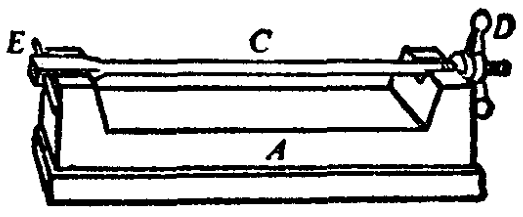
\includegraphics[width=5.5cm]{../pic/czwl2-ch2-4}
    \caption{冷缩时产生的力}\label{fig:2-4}
\end{wrapfigure}

在坚固的生铁座架 $A$上放一根烧得很热的钢棒 $C$ (图 \ref{fig:2-4})。
钢棒的一头有一段生铁棍 $E$,另一头有一个螺旋 $D$ 可以使钢棒卡紧在座架上。
当钢棒冷却收缩时,生铁棍便被拉断。

各种技术设备的温度都要随着气温或工作情况而改变,这就需要我们采取一些办法,
来防止热胀冷缩产生的力的破坏作用。在铺设铁轨的时候,两根铁轨接头的地方要留空隙。
长的铁桥只是一端固定,另一端要架在滚子上(图 \ref{fig:2-5})。这样,当气温变化的时候,
铁轨和铁桥都可以自由伸缩,不致损坏。
工厂里,蒸汽导管的中部装有弯曲的伸缩管(图 \ref{fig:2-6}),当导管里通过高温蒸汽的时候,
导管受热伸长,伸缩管的弯曲程度就改变,使导管不致损坏。

\begin{figure}[htbp]
    \centering
    \begin{minipage}{9cm}
    \centering
    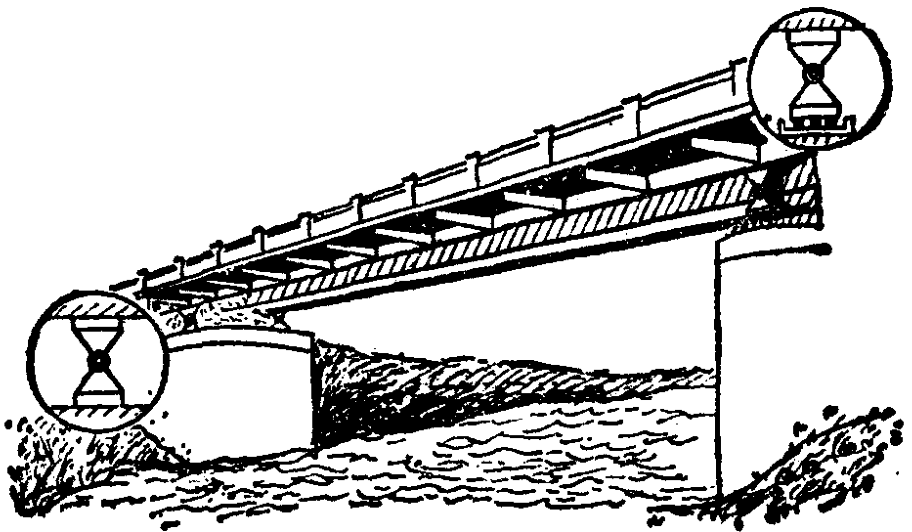
\includegraphics[width=7cm]{../pic/czwl2-ch2-5}
    \caption{铁桥右端架在滚子上}\label{fig:2-5}
    \end{minipage}
    \qquad
    \begin{minipage}{5cm}
    \centering
    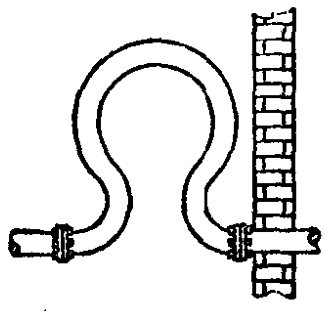
\includegraphics[width=4cm]{../pic/czwl2-ch2-6}
    \caption{伸缩管}\label{fig:2-6}
    \end{minipage}
\end{figure}

技术上也常常利用固体的热膨胀来做有益的事情。
例如,为了使火车车轮耐用,在轮上要套一个硬度大、耐磨损的轮箍。
为了套得紧密,轮箍的内径要做得比车轮稍小一些。
在套轮箍的时候,先把轮箍烧得很热,使它的内径膨胀得比轮子稍大,
然后套在轮子上,轮箍冷却收缩后,就紧紧地箍在车轮上了。
把滚珠轴承装到钢轴上,通常也采用类似的方法,先把轴承浸入热油里,
使它的内径膨胀得比钢轴稍大,然后套在钢轴上。

\begin{wrapfigure}[10]{r}{6cm}
    \centering
    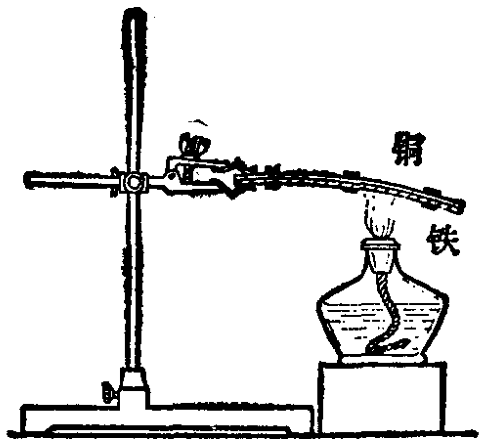
\includegraphics[width=5.5cm]{../pic/czwl2-ch2-7}
    \caption{双金属片}\label{fig:2-7}
\end{wrapfigure}

在相同的条件下,物体的材料不同,热膨胀的大小一般也不相同。
这可以从下面的实验看出来。
把长和宽都相同的铜片和铁片紧紧地铆在一起,做成双金属片。
用酒精灯给双金属片加热,双金属片就向铁片那边弯曲(图 \ref{fig:2-7}),
这表明当同样受热时,铜片膨胀得比铁片大。

各种仪器、机器、建筑物通常都是用不同的材料制成的。
选择这些材料时,必须考虑到它们的热膨胀是不是一样。
例如,在电灯泡上,焊接在玻璃中的那部分金属线,它的热膨胀必须跟玻璃的相等,
这样,温度改变时,金属线和玻璃之间的接合才不会松脱,金属线也不会把玻璃胀破。
在钢筋混凝土建筑物中,钢筋和混疑土的热膨胀也要相同,不然,建筑物就不可能坚固。


\lianxi

(1) 夏天,自行车轮胎里的气如果打得太足,在太阳暴哂下,轮胎容易爆破。为什么?

(2) 乒乓球瘪进去一块,把它浸入开水里烫一下会重新鼓起来。为什么?

(3) 壶里装满冷水,放在火上加热,水会从壶里溢出来。为什么?

(4) 汽油、柴油通常是装在密封的油桶里运输或贮存的。
在向油桶里装油时总要留些空隙,不能装得满满的。为什么?

(5) 为什么混凝土马路每隔一定的距离要留一道缝隙?

(6) 举出两个你知道的利用或防止物体热膨胀的例子。



\section*{小实验}

利用双金属片受热时弯曲的现象,你可以自己做一个自动控制电路。

\begin{figure}[htbp]
    \centering
    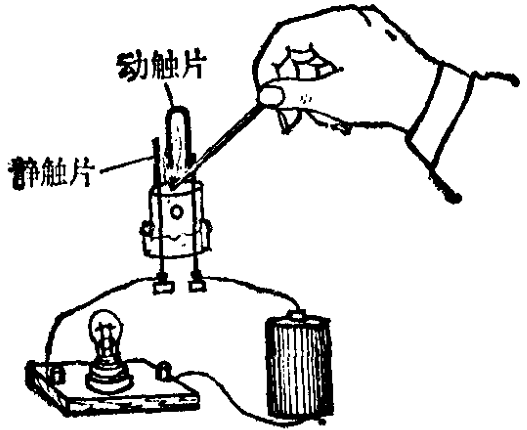
\includegraphics[width=0.5\textwidth]{../pic/czwl2-ch2-8}
    \caption{}\label{fig:2-8}
\end{figure}

找一个废的日光灯起动器,去掉金属(或塑料)外壳,再小心地把玻璃泡打破(注意不要把下边的金属线弄断),
就露出了它的静触片和动触片(图 \ref{fig:2-8})。 U 形的动触片就是双金属片。
照图上画的那样,用导线把起动器、小灯泡和电池连接起来。
点燃火柴去烧动触片,它受热变形跟静触片相接触,于是小灯泡亮了起来。
火柴熄灭后,动触片变冷离开静触片,又恢复到原来的位置,小灯泡就不亮了。

想想看,动触片里面和外面的两种金属,哪一种受热时膨胀得大?

实验中遇到的电路问题,学了电学以后,就会明白了。


